%% Adapted from `tikzposter-example.tex',

%% Modify the size of the paper for the usual 4 ft x3 ft poster size
\PassOptionsToPackage{paperwidth=48in, paperheight=36in,
  textwidth=48in, textheight=36in,
  innermargin=1in, margin=.25in,
  centering}{geometry}
\PassOptionsToPackage{dvipsnames}{xcolor}
\documentclass[25pt, landscape,blockverticalspace=0.5in, colspace=0.5in, subcolspace=0.33in]{tikzposter} %Default values for poster format options.
\tikzposterlatexaffectionproofoff % remove tikzposter logo

%% fonts: helvetica + palatino
% Euler for math | Palatino for rm | Helvetica for ss | Courier for tt
\renewcommand{\rmdefault}{ppl} % rm
\linespread{1.05}        % Palatino needs more leading
\usepackage[scaled]{helvet} % ss
\usepackage{courier} % tt
%\usepackage{euler} % math
\usepackage{eulervm} % a better implementation of the euler package (not in gwTeX)
\normalfont
\usepackage[T1]{fontenc}
\renewcommand{\familydefault}{\sfdefault} % use sans-serif

%%%% OTHER IMPORTANT PACKAGES
\usepackage{amsmath, amsthm, amssymb} %AMS math
\usepackage{bm}% bold math
\usepackage{color} % colored text
\usepackage[pdftex,colorlinks=true,
allcolors=blue
]{hyperref}% add hypertext capabilities
\usepackage{paralist}% for compactitem used by Marko
\usepackage{multirow}% multicolumn/row cells in tables
\usepackage{url} % add auto-linked urls
\usepackage{mathtools} % shortintertext, and other useful math-related features
\usepackage{siunitx} % SI units
\sisetup{per-mode = symbol}
\usepackage[dvipsnames]{xcolor}
\usepackage{pgfplots}
\pgfplotsset{compat=newest}

\usetikzlibrary{calc} % relative positioning of nodes
\usetikzlibrary{arrows.meta} % for arrow annotations
\tikzstyle{arrow}+=[<-,line width=4pt, >={Latex[width=.2in,length=.2in]}, color=colorOne]
\tikzstyle{bubble}+=[anchor=west,color=colorOne,right,text width=2in,fill=white, fill opacity=0.75, text opacity=1,draw]


% choose one bibliography package:
\usepackage[backend=bibtex,citestyle=numeric-comp]{biblatex}
%\usepackage{amsrefs} % references
%%%%

\addbibresource{bibliography.bib} % bibliography file

% Title, Author, Institute
\title{A most excellent research project}
\author{First Author$^1$, Second Author$^2$}
\institute{${}^1$ Clarkson, ${}^2$ Not Clarkson}

 \begin{document}

 %% header
 \maketitle
 \node[anchor=west] at (TP@title.west) {\hspace{3in}
\includegraphics[height=3in]{logos/clarkson-seal.png}};
 \node[anchor=east] at (TP@title.east) {
\includegraphics[height=2in]{logos/clarkson-logo.png} \hspace*{2in}};


 \begin{columns}%blocks will be placed into columns
       \column{.33}
       \block{Title}{
         Math:
         \[
           \int_0^t f(x(\tau))d\tau
         \]

         We can also put a graph in and refer to it here: Fig.~\ref{fig:first}
         \begin{tikzfigure}[This is a graph.]\label{fig:first}
           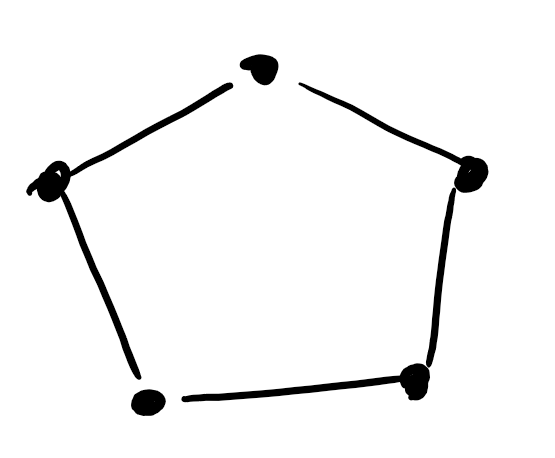
\includegraphics[width=0.5\linewidth]{figs/graph}
         \end{tikzfigure}
       }
       \column{.33}
       \block{Methods}{
         Something common.
         \coloredbox{Important statement can be highlighted}
       }
       \begin{subcolumns}
         \subcolumn{.5}
         \block{Type 1}{
           Something cited from
           \cite{Hill1894}
         }
         \subcolumn{.5}
         \block{Type 2}{
           Something else}
       \end{subcolumns}
       \block{More}{
         For more information, take a look at \texttt{tikzposter-example.tex} and \texttt{tikzposter-example.pdf} in this folder.
       }
       \note[targetoffsetx=2in, angle=-45,targetoffsety=0in,connection]{Additionally, documentation for the poster class is in \url{https://ctan.org/pkg/tikzposter}.}


       \column{.33}

       \block{Results}{


\begin{tikzfigure}[Title]
   \begin{tikzpicture}
     \begin{axis}[
       xmin=0, xmax=6,
       xlabel={$x$},
       ymin=0, ymax=6,
       ylabel={$y$},
       axis lines=middle,
       axis line style=->,
       width=.9\linewidth]
        \addplot[no marks,blue,-,domain=0:6, samples=100] expression{sqrt(x)};
        \addlegendentry{$y=\sqrt{x}$};
      \end{axis}
   \end{tikzpicture}
 \end{tikzfigure}

 On posters, adding annotations to graphs is a very effective way to communicate what is displayed AND at the same time reduce the amount of text. For more annotation examples, see the end of the document
 
      \draw[arrow,->] (15,8) % head of arrow (notice the arrow symbol after \draw command)
     -- node [text width=1.5in,midway,above,left] {Annotation 3}
     +(45:8); % 45 degrees, length = 8

}

       \block{References}{
         \printbibliography[heading=none]
       }

     \end{columns}

%% Annotations
% default styles for "arrow" and "bubble" are defined just above "\begin{document}"
% search for commands \tikzstyle
%
%  On posters, adding annotations to graphs is a very effective way to communicate
%  what is displayed AND at the same time reduce the amount of text. For more
%  annotation examples, see the end of the document

     \draw[arrow,<->] (12,11) % tail of arrow
     node[bubble] {Annotation 1} % annotation text
     -- % line
     +(-150:3); % tip of arrow: angle 135, length=2

     \draw[arrow] (10,-16) %anchor point - experiment to see how the coordinates move
     -- % line
     +(45:3) % arrow leaves the anchor at 45 degrees and continues for 3 units
     node[bubble, text width=3in] {Annotation Example: See end of LaTeX document}; % annotation text



 \end{document}




\endinput
%%
%% End of file `tikzposter-example.tex'.
